\documentclass{article}
\usepackage[T1]{fontenc}
\usepackage[french]{babel}
\usepackage{csquotes}
\usepackage{amsmath}
\usepackage{graphicx}
\usepackage{booktabs}
\usepackage[style=authoryear]{biblatex}
\addbibresource{references.bib}
\usepackage[colorlinks=true, allcolors=blue]{hyperref}

\title{{{TITLE}}}
\author{{{AUTHOR}}}
\date{\today}

\begin{document}

\maketitle

\begin{abstract}
Ce projet exemple montre en quelques pages ce qu'on écrit le plus souvent
avec \LaTeX{}: des sections, une figure, un tableau, des listes, des
mathématiques et des références. Modifiez-le à votre guise.
\end{abstract}

\section{Pour commencer}

Le code \LaTeX{} est à gauche et le PDF à droite. Pour mettre le PDF à jour,
cliquez sur le bouton de compilation ou appuyez sur Ctrl+Entrée (Cmd+Entrée
sur Mac). Un double-clic dans le PDF amène à la ligne correspondante du code.

\subsection{Sections et sous-sections}

Les commandes \verb|\section| et \verb|\subsection| découpent le texte. Elles
sont numérotées automatiquement et \verb|\tableofcontents| en fait la table
des matières.

\section{Figures}

La figure~\ref{fig:courbes} affiche l'image \texttt{images/courbes.png} du
projet. Pour ajouter les vôtres, téléversez-les dans le dossier
\texttt{images} ou utilisez le bouton \enquote{Insérer une figure} de la
barre d'outils.

\begin{figure}[htbp]
  \centering
  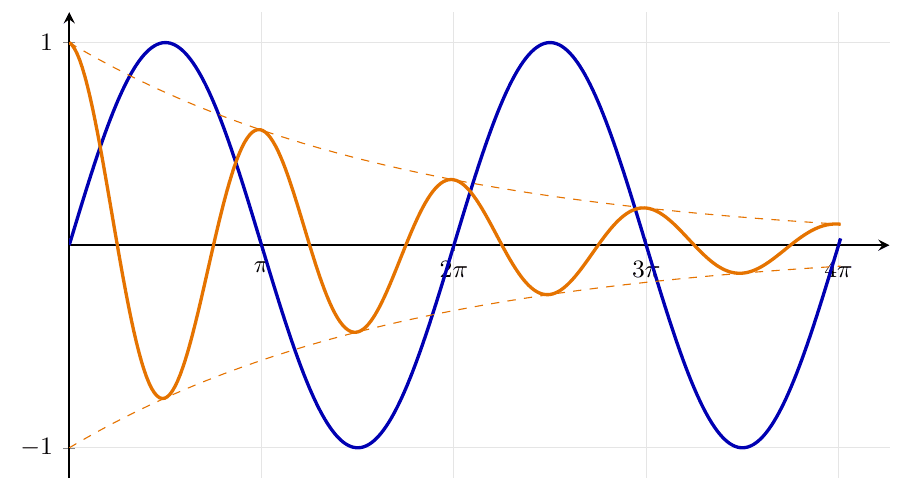
\includegraphics[width=0.8\linewidth]{images/courbes.png}
  \caption{Une sinusoïde et une oscillation amortie.}
  \label{fig:courbes}
\end{figure}

\section{Tableaux}

Le tableau~\ref{tab:mesures} utilise les filets de l'extension
\texttt{booktabs}.

\begin{table}[htbp]
  \centering
  \caption{Quelques mesures.}
  \label{tab:mesures}
  \begin{tabular}{lrr}
    \toprule
    Essai & Durée (s) & Température (°C) \\
    \midrule
    A & 12,5 & 21,3 \\
    B & 14,1 & 22,8 \\
    C & 11,9 & 20,6 \\
    \bottomrule
  \end{tabular}
\end{table}

\section{Listes}

Une liste à puces:
\begin{itemize}
  \item des éléments sans ordre particulier;
  \item que l'environnement \texttt{itemize} présente.
\end{itemize}
Une liste numérotée:
\begin{enumerate}
  \item une première étape;
  \item puis une seconde, avec \texttt{enumerate}.
\end{enumerate}

\section{Mathématiques}

Les formules s'écrivent dans le texte, entre dollars, comme $E = mc^2$, ou
centrées et numérotées:
\begin{equation}
  \int_0^{\infty} e^{-x^2} \, \mathrm{d}x = \frac{\sqrt{\pi}}{2}.
  \label{eq:gauss}
\end{equation}
L'équation~\eqref{eq:gauss} est l'intégrale de Gauss. L'environnement
\texttt{align} aligne plusieurs lignes:
\begin{align}
  (a + b)^2 &= a^2 + 2ab + b^2, \\
  (a + b)(a - b) &= a^2 - b^2.
\end{align}

\section{Marges et format du papier}

L'extension \texttt{geometry} règle le format du papier et les marges. Par
exemple, dans le préambule:
\begin{verbatim}
\usepackage[letterpaper, margin=2.5cm]{geometry}
\end{verbatim}
Remplacez \texttt{letterpaper} par \texttt{a4paper} pour le format A4.

\section{Références}

Les références se trouvent dans \texttt{references.bib}. On les cite avec
\verb|\textcite| ou \verb|\parencite|: \textcite{knuth1984} a créé \TeX{},
puis \textcite{lamport1994} a écrit \LaTeX{} par-dessus. La bibliographie se
compose seule à la fin du document \parencite{mittelbach2023}.

\printbibliography

\end{document}
